\section{Zeitplan}

% Zeitplan
% - 2018 - 2040 Umstellung der Nationalen Ökonomie
% - 2040 - * Zeitraum für die Stärkung von Senken für 
%   Treibhausgasen im nationalen, europäischen und
%   globalen Rahmen
Die Zeit für eine umfängliche Reduktion der Treibhausgasproduktion in Gesellschaft, Industrie, Landwirtschaft, Transport und der Energieerzeugung ist knapp bemessen.
Die verbleibende Restmenge an CO\textsubscript{2}-Ausstoß-Äquivalenten beträgt 1500 Gt CO\textsubscript{2} und muss nahezu vollständig vermieden werden (vgl. \autoref{fig:co2-reduction}).
Neben der Vermeidung von CO\textsubscript{2} sind auch mit Maßnahmen des Climate-Engineering notwendig um unsere Klimaziele zu erreichen und u.a eine Negativemission ab 2050 zu erreichen.
Je früher größere CO\textsubscript{2}-Reduktionen erreicht werden, desto länger ist es möglich in kritischeren, schwer änderbaren Bereichen noch länger CO\textsubscript{2} zu produzieren.

\begin{figure}[!htb]
	\centering
	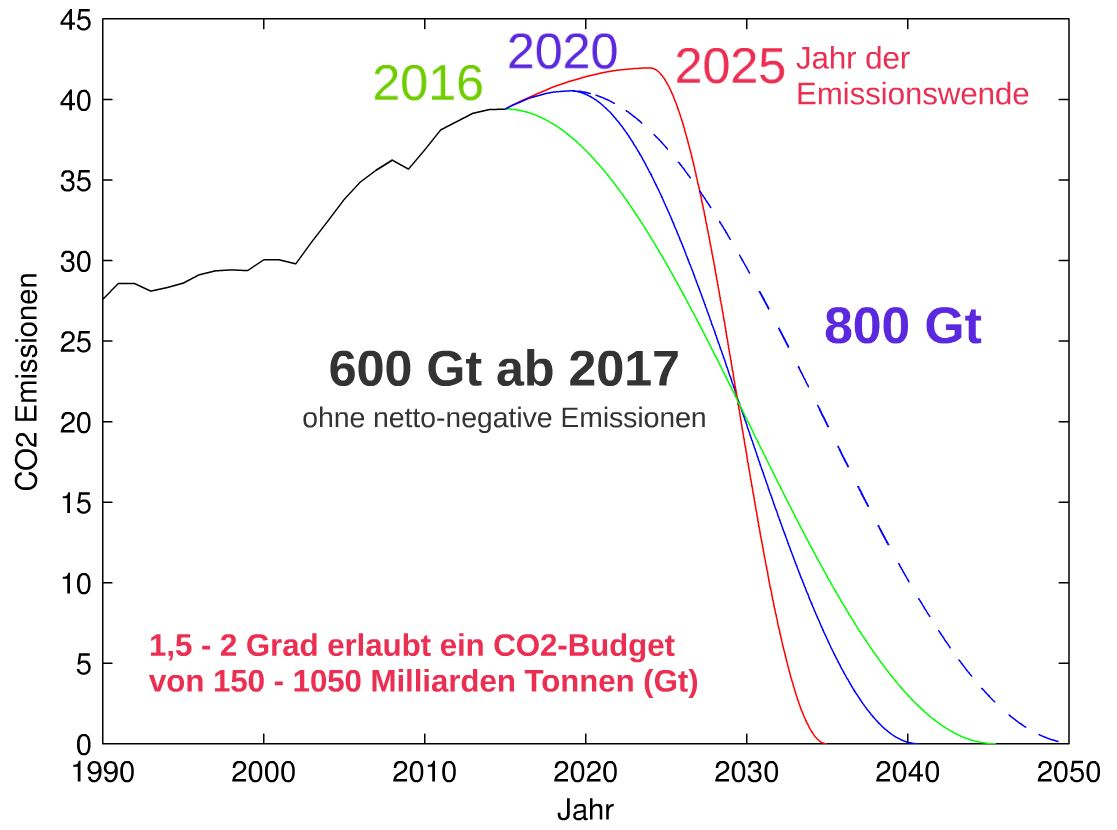
\includegraphics[width=0.8\textwidth]{emission-paths-for-reaching-the-paris-agreement.jpg}
	\caption{Nötige Emissionspfade um das Übereinkommen von Paris einzuhalten}
	\label{fig:co2-reduction}
\end{figure}

Wie \autoref{fig:co2-reduction} zu entnehmen ist, führt eine zögerliche Umsetzung dazu, dass uns weniger Zeit für die Umstellung bleibt.
Es ist deshalb erforderlich, die leicht erreichbaren Ziele zeitnah -- in den nächsten 5 Jahren -- anzustreben um so Zeit zu gewinnen um komplexere Maßnahmen umzusetzen.





